\chapter{Schedule Transformations}\label{chap:RAJALC}

Typical parallelization approaches such as OpenMP and CUDA provide constructs for parallelizing and blocking for data locality for individual loops.
By focusing on each loop separately, these approaches fail to leverage sources of data locality possible due to inter-loop data reuse.
The loop chain abstraction provides a framework for reasoning about and applying inter-loop optimizations.
In this chapter, I incorporate the loop chain abstraction into RAJA, a performance portability library for high-performance computing applications.
Using the loop-chain-extended RAJA, or RAJALC, developers can have the RAJA library apply schedule transformations like loop fusion and overlapped tiling while maintaining the original structure of their programs. 
By introducing targeted symbolic evaluation capabilities, RAJALC can collect and cache data access information required to verify loop transformations.
I evaluate the performance improvement and refactoring costs of other extension.
Overall, the results demonstrate 85--98\% of the performance improvements of hand-optimized kernels with dramatically fewer code changes.

\section{Introduction and Summary}
Scientific inquiry leverages high-performance computing (HPC) for a variety of
tasks, including data analysis and experiment design. 
Also, experiments are often performed \textit{in silico}, using 
simulation instead of real-world experiment.
Further, the rise of machine learning gives HPC principles wider
applicability than ever before.

HPC systems are incredibly diverse architecturally, 
both in terms of compute and data.
The ten fastest HPC systems use nine different processor/coprocessor
configurations~\cite{top500}.
This architectural diversity implies that applications designed to be
performant on one system do not necessarily perform well on others.
%Sorta C1
Because the labor costs of developing a new version of an application are so high, 
there is a need for tools that allow developers to design a single application
that performs well across systems with minimal modifications.

Performance portability libraries like RAJA~\cite{hornung2014RAJA} do exactly this.
These libraries enables programmers to specify loops with templated functions,
where one template parameter is an execution policy that describes how a computation should be run.
In RAJA, examples of these policies include \verb.simd_exec. (vectorized), \verb.omp_parallel_for_exec. (OpenMP threading), or \verb.cuda_exec. (GPU).
Thus the heavy lifting of porting a parallel implementation to different 
architectures is abstracted into standardized execution policies.


When optimizing an application, loops are generally considered and
parallelized one at a time.
Optimizing the performance of HPC applications is more complicated than introducing new parallelism.
Many applications are not compute-bound, meaning additional parallelism does not improve performance. 
Instead, moving data to and from memory and accelerators bottlenecks these applications. 
While PPLs support porting per-loop parallelism between systems, they lack the ability to port inter-loop schedule transformations that improve data locality. 
The key capability they need to enable porting these transformations is an inter-loop scope.
The loop chain abstraction provides exactly this.

The loop chain abstraction~\cite{krieger2013loop} captures sequences of loops that share 
data and enough information about how such loops access 
data to enable inter-loop optimization.
Considering loops as a chain uncovers optimizations, like fusion
and overlapped tiling, that are impossible to replicate when optimizing
each loop independently.
\textbf{I address the problem in porting data locality optimizations in this
work by incorporating loop chaining, an abstraction for balancing data locality
with parallelism across loops, into a representative performance portability library, RAJA.}
The technique imposes a minimal code delta on the developer, leverages C++'s
operator overloading and generic lambdas to perform necessary analysis, and
requires no additional compilation steps.

This chapter presents the following contributions:
\begin{itemize}
\item the design of a compact RAJA extension to enable inter-loop
			optimizations;
\item a methodology to perform symbolic evaluation in C++ code;
\item an implementation of these techniques in RAJA\@; and
\item evaluation of their porting costs and performance benefits.
\end{itemize}

For the RAJAPerf case study, RAJALC requires 8.5 source lines of code changed or added on average, compared to 23.625 when implementing by hand.
Furthermore, in 21 of 24 benchmark-system combinations, RAJALC sees performance changes in the same direction as hand-implemented variants, and 85--98\% of the performance improvement, depending on the system.

\section{RAJA's Approach to Portability}

Before making the step to inter-loop representation and optimization, let us the key features of RAJA that enable performance portability
as RAJALC leverages them.
These features are an abstraction layer for data accesses and the
orthogonal specification of loop schedules
(i.e., separating the specification of the loop body from the loop iteration).
Current usage of RAJA leverages these for loop parallelization and
data layout transformations.
In this paper, I use these features to build the loop chain abstraction.

\subsection{RAJA HYDRO\_2D Example}
%First person plural bc its me and the reader walking through stuff
To illustrate the loop and data access abstraction and to provide context
for the required coding effort, I port a loop in the HYDRO\_2D benchmark
from its reference C/C++ implementation to use RAJA\@.
Listing~\ref{hydroPort} shows the before and after for the port.

RAJA has two built-in execution primitives: \verb.forall. and \verb.kernel..
\verb.forall. is used for unnested loops, so for this example we use
\verb.kernel..
We must provide three pieces of information to \verb.kernel.. 
First, we provide the execution policy, which describes the structure of
the loop and what parts to run in parallel.
Second, we provide a container of iterator tuples, which describe the
iterator values for the loop execution.
Last, we provide a lambda function that describes the loop body.


Another useful step employs RAJA's array wrapper, the View, which supports
easily changing the layout of arrays.
Their use is generally optional with RAJA, but is required to use the loop
chain abstraction.
The abstraction requires data access information, which we collect by
overloading View operators.
Lines 10--11 of Listing~\ref{hydroPort} show how to initialize \verb.zrout.
as a View object.

\begin{figure}
\begin{lstlisting}[label={hydroPort},
    caption={Hydro\_2D Loop (Color indicates code regions of original and RAJA versions that perform similar functions)}]
//original loop nest
<@\textcolor{red}{for}@>(<@\textcolor{blue}{Index\_type k = kbeg; k < kend; k++}@>) {
  <@\textcolor{orange}{for}@>(<@\textcolor{violet}{Index\_type j = jbeg; j < jend; j++}@>) {              
    <@\textcolor{ForestGreen}{zrout[k][j] = zr[k][j] + t * zu[k][j];}@>
    <@\textcolor{ForestGreen}{zzout[k][j] = zz[k][j] + t * zv[k][j];}@>
  }
}

//initializing View objects, (one for each array)
<@\textcolor{black}{using VIEW\_TYPE = View<double, Layout<2> >;}@>
<@\textcolor{black}{VIEW\_TYPE zrout(new double [kN * jN], kN, jN);}@>


<@\textcolor{black}{using}@> KPol = KernelPolicy<
  <@\textcolor{red}{statement::For<0, RAJA::loop\_exec,}@>
    <@\textcolor{orange}{statement::For<1, RAJA::loop\_exec,}@>
      <@{\textcolor{ForestGreen}{statement::Lambda<0>}@>
    >
  >
>;

kernel<KPol>(make_tuple(<@\textcolor{blue}{RangeSegment(kbeg, kend)}@>,
                           <@\textcolor{violet}{RangeSegment(jbeg, jend)}@>),
               <@\textcolor{ForestGreen}{[=] (int k, int j) \{}@>
                 <@\textcolor{ForestGreen}{zrout(k,j) = zr(k,j) + t * zu(k,j);}@>
                 <@\textcolor{ForestGreen}{zzout(k,j) = zz(k,j) + t * zv(k,j);}@>
              <@\textcolor{ForestGreen}{ \}}@>);
\end{lstlisting}
\end{figure}

\subsection{Impact of RAJA}

RAJA provides a methodology to improve application portability.
As the high end of high performance computing transitions from traditional
homogeneous core designs into heterogeneous systems, applications 
require a common abstraction to keep up with the variety of platforms
and their associated programming models.
RAJA provides that abstraction for LLNL C++ applications, which are large
(i.e., a hundred thousand to low millions of lines), long lived (i.e., often
20 years or greater), and must both run and perform well on cutting-edge
hardware to accomplish their goals.

RAJA has grown into a library that implements the core constructs and
architecture and model-specific policies, across a myriad of platforms and
backends. RAJA is in production use in eight~\cite{raja-ecp-report} distinct
LLNL applications and libraries, as well as several ECP applications including
SW4~\cite{sw4}, GEOSX~\cite{geosx}, and SUNDIALS~\cite{sundials}.

Results published for three LLNL production codes~\cite{raja-p3hpc} show
performance portability across a variety of architectures.  Comparing a whole
node to a whole node, Ares achieved $13\times$, ALE3D achieved $17\times$ and
Ardra achieved $12\times$ speedups on nodes of the LLNL Sierra system for
meaningful inputs.


\section{Loop Chain Abstraction}\label{sec:loopchain}
RAJA loop execution policies apply to individual loops.
Often two or more loops exhibit producer/consumer data sharing.
The loop chain abstraction~\cite{krieger2013loop} enables scheduling
across such loops to improve temporal data locality. 
The goal is to design RAJA techniques to express and to schedule loop chains.

\subsection{Loop Chains}

A loop chain is a sequence of loop nests $L_{0},L_{1},L_{2},\dots,L_{n}$,
in which each loop nest $L_{i}$ has four associated components:
\begin{itemize}
\item an iteration space $I_{i}$,
\item functions $R_{i}$ and $W_{i}$ that map iteration $i$ to the data 
      elements that it reads and writes;
\item a parallelism policy $p_{i}$ that describes how the loop can be executed; and
\item a loop body $B_{i}$.
\end{itemize} 

The loop chain abstraction expands the possible loop scheduling scope.
Using it to optimize an application consists of three stages:
specifying loop objects; specifying or selecting provably correct loop
transformations; and applying those transformations.

\subsection{Loop Chain Transformations}

Every loop nest has a schedule that describes the order in which the 
iterations should execute.
A lexicographical ordering over integer vectors that represent the
iterations describe this schedule.
Consider the loops in Listing~\ref{scheduleVector}, which sum array
\ttt{a} into \ttt{b} and then store a stencil computation on \ttt{b}
into \ttt{c}.

\begin{figure}[t]
	\begin{lstlisting}[label={scheduleVector},caption={Example Loop Chain}]
	for i = 0 to N:
		for j = 0 to M:
			b[i][j] += a[i][j]                     // B0
	for i = 1 to N-1:
		for j = 1 to M-1:
			c[i][j] = b[i-1][j] + b[i][j] + b[i+1][j] / 3;     // B1
	\end{lstlisting}
	\end{figure}


The set $I_{0}=\{[0,i,0,j,0] \; | \; 0 \leq i < N, 0 \leq j < M\}$ describes
the iterations of the first loop while the set of vectors
$I_{1} = \{[1,i,0,j,0] \; | \; 1 \leq i < N-1, 1 \leq j < M-1\}$ describes
those of the second.
Within each tuple, the first element is the loop index, the second and fourth are the iteration of the loop dimensions, and the third and fifth are the statement index within the loop. 
We can describe the sequential loop schedules as the lexicographical ordering over
$\mathbb{Z}^{5}$.

Legal loop transformations and schedules must respect the data dependences
in the program~\cite{frameworkKP95pub}.
These data dependences can be described as relations over the iterations 
of loops.
The example has dependences from the first statement, $B0$, to the second,
$B1$, due to the writes to \ttt{b} in the first loop and the reads from
\ttt{b} in the second. 
The relations $D_{i-1} = \{[0,i,0,j,0] \to [1,i-1,0,j,0]\}$,
$D_{i} = \{[0,i,0,j,0] \to [1,i,0,j,0]\}$, and
$D_{i+1} = \{[0,i,0,j,0] \to [1,i+1,0,j,0]\}$ describe those dependences. 
The relation induced by the read from \ttt{b[i-1][j]} 
%results in $i+1$
%in the relation because 
is due to the data element written in iteration (i,j) of the
first loop being read by iteration $(i-1,j)$ of the second loop. %, not $(i-1,j)$.
%Write-after-write and write-after-read dependences are formulated similarly.

A legal loop transformation maintains dependence relations. 
That is, a transformation is legal if its application to the dependence
relations remains a subset of the schedule relation.
Consider the fusion transformation on the example loops, which maps the
iteration vectors of the second loop from $[1,i,0,j,0]$ to $[0,i,0,j,1]$. 
Its application to the dependence relation $D_{i-1}$ yields
$\{[0,i,0,j,0] \to [0,i-1,0,j,1]\}$.
Thus, $x > y$ in the schedule for any pair of iterations $(x,y)$ that
$D_{i-1}$ relates, and so the transformation is not legal.

The loop chain abstraction uses the information associated with each loop 
nest to build these representations.
The iteration spaces $I_{i}$ and loop bodies $B_{i}$ describe the iteration
vectors; the data access functions $R_{i}$ and $W_{i}$ construct the
dependence relations; and the parallelism policies $p_{i}$ inform the
schedule relations.


\subsection{Loop Objects in RAJA}

Although RAJA does not intrinsically provide chainable loop objects, it has many
of the necessary components.
The execution primitive and common case, \ttt{kernel} and  \ttt{forall}, form
the initial basis for the description of loop nests.
The first kernel argument is a collection of iterator tuples, an explicit
instance of an iteration space.
The parallelism policy is found in the kernel policy template argument.
The loop body is a variable-length list of lambda functions.
This leaves only two data access functions, which are implicitly encoded
within the loop body.
Section~\ref{subsec:accesses} describes the symbolic evaluation extension
that extracts them.

\section{Design Changes to RAJA}

First, I introduce an interface in RAJA for users to specify loop chains and transformations
so as to enable inter-loop optimizations without additional tooling or compilation steps.
Second, I design a symbolic evaluation mechanism that gathers data access patterns of
kernels.
Third, I use this mechanism to analyze kernels at runtime and use the results to automate the generation of a safe execution schedule for the kernels.


Traditional polyhedral optimization techniques are normally broken up into identifying code regions to optimize, converting to a polyhedral representation, analyzing the structure, applying transformations, and generating code.
Because RAJALC operates at the language level rather than the compiler level, my approach is slightly different. While identifying code regions, converting to a polyhedral representation, and analysis are roughly equivalent to compiler-level approaches, transformation and code generation are formulated differently. 
The fundamental difference is that transformation and code generation happen \textit{before} any analysis.

\subsection{RAJA Computations as Objects}
\begin{figure}[t]
	\begin{lstlisting}[caption={Using the \texttt{fuse} and \texttt{overlapped\_tile} transformations.}, label={transformExample}]
	auto lambda1 = [=](auto i) {c(i) = a(i) * b(i);};
	auto lambda2 = [=](auto i) {d(i) = d(i) + c(i);};
	
	auto loop1 = make_forall<simd_exec>(RangeSegment(0,N), lambda1);
	auto loop2 = make_forall<simd_exec>(RangeSegment(0,N), lambda2);
	
	auto fused = fuse(loop1, loop2);
	fused();
	
	
	auto lambda3 = [=](auto i) {b(i) = (a(i-1) + a(i) + a(i+1) ) / 3;};
	auto lambda4 = [=](auto i) {c(i) = (b(i-1) + b(i) + b(i+1) ) / 3;};
	
	auto loop3 = make_forall<...>(RangeSegment(1,N-1), lambda3);
	auto loop4 = make_forall<...>(RangeSegment(1,N-1), lambda4);
	
	//default tile size
	auto tiled_default = overlapped_tile(loop3, loop4);
	//tile size = 64
	auto tiled_64 = overlapped_tile<64>(loop3, loop4);
	tiled_64();
	 \end{lstlisting}
	\end{figure}
Delayed execution is a key design pattern in %optimizing languages like
embedded domain-specific languages such as
Halide~\cite{ragan-kelley2013halide} and Tensorflow~\cite{tensorflow}.
These languages separate the statements that specify a computation from
those that execute it.
In between, the programmer can specify how to schedule and optimize the computation.
However, in standard RAJA, computational \verb.kernel. statements immediately execute the specified computation.
So, I introduce a wrapper class (\verb.KernelWrapper.) that enables execution
to be delayed until after analysis and transformation.
I introduce two functions based on existing kernel execution functions to
create \verb.KernelWrapper.s: \verb.make_forall. and \verb.make_kernel..
They have the same interface as their corresponding execution functions, but
return a \verb.KernelWrapper. object that can be executed or optimized.
Listing~\ref{transformExample} shows these wrapping functions in use. 


\subsection{Gathering Access Information}\label{subsec:accesses}
\begin{figure}[t]
\begin{lstlisting}[label={symExecChanges}, caption={Kernel Lambda Conversion}]
auto original_lambda = [=](idx_t i, idx_t j) {
	a[i][j] += b[i][j];
};

auto converted_lambda = [=](auto i, auto j) { //idx_t -> auto
	a(i,j) += b(i,j); // array -> View
};
\end{lstlisting}
\end{figure}

\begin{figure}
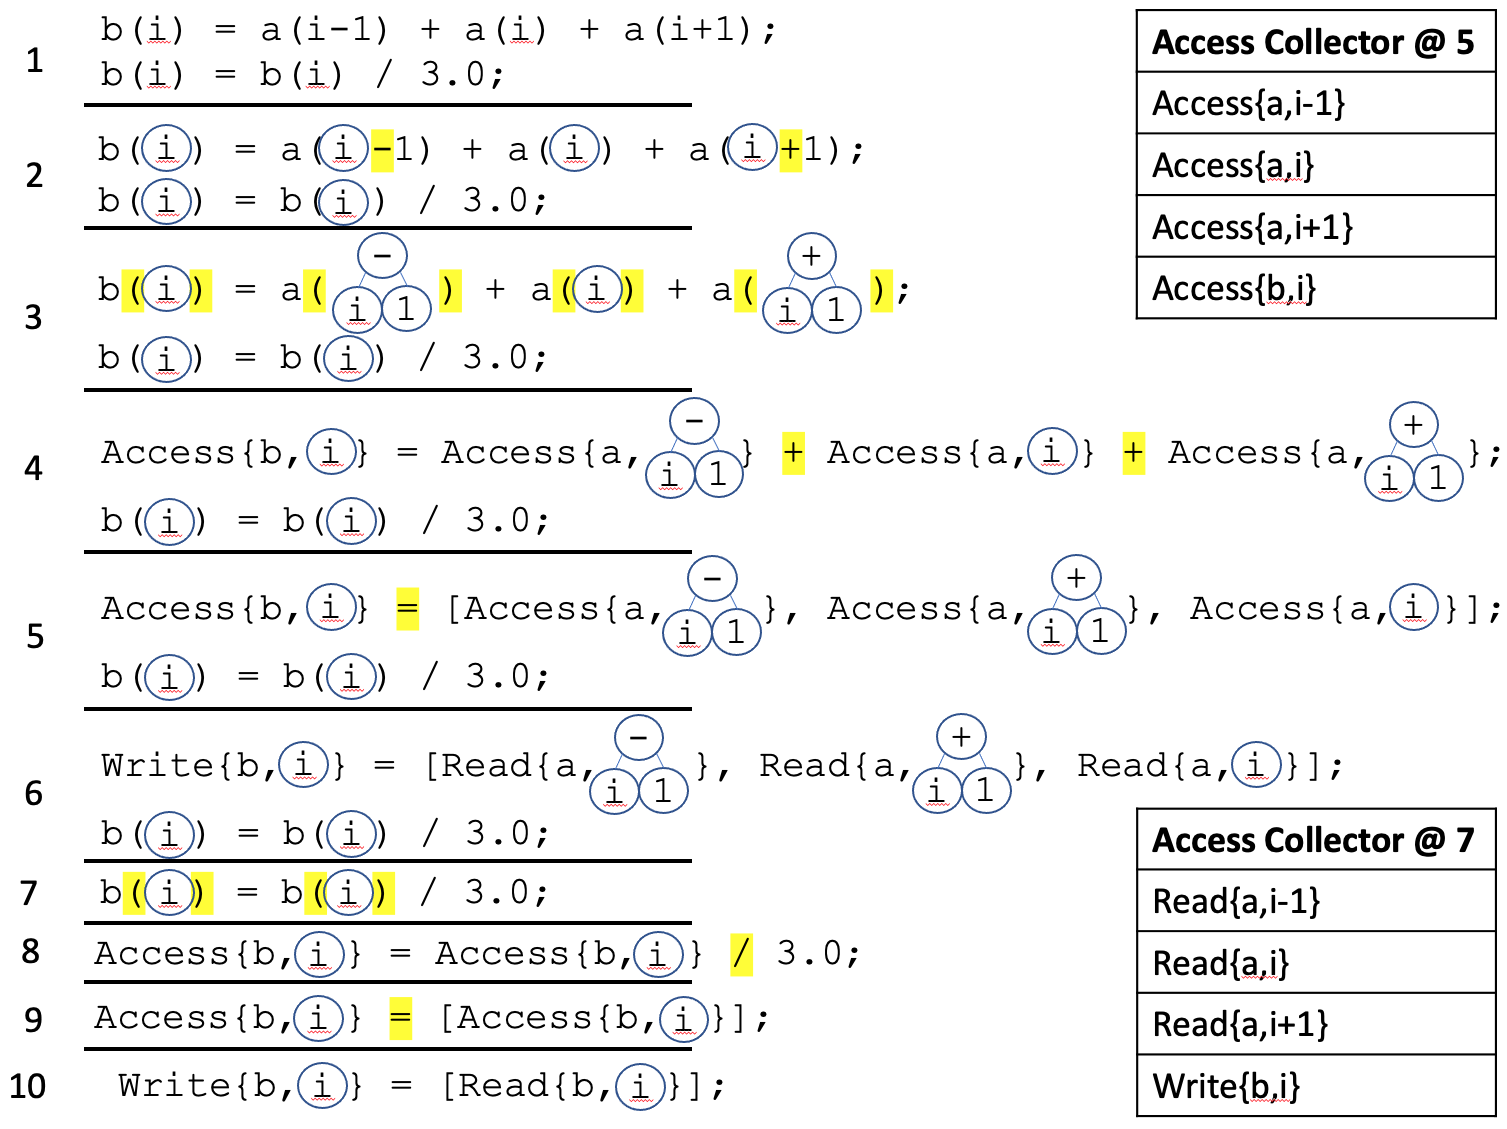
\includegraphics[width=\linewidth]{SymExecProcess.png}
\caption{Symbolic evaluation of a kernel lambda. 
Indexing expressions are evaluated first, then accesses, then statements in terms of accesses.
As assignments are evaluated, the accesses are marked as reads or writes.
Accesses are tracked using the access collector.}\label{symExec}
\end{figure}
Specifying parallelism within RAJA and other programming models can
build on commonly used abstractions such as \verb.forall..
However, determining when inter-loop scheduling transformations such as
loop fusion are legal requires an analysis of the dependences between those loops.
%Data access information is the largest missing piece for enabling loop chains
%in RAJA.
Other loop chain approaches require specification of data access patterns by
hand, which effectively rewrites the loop~\cite{bertolacci2019using}.
The symbolic evaluation mechanism eliminates this effort for the
developer by leveraging RAJA's array wrapping View abstraction.

%We leverage RAJA's array wrapping Views, which use the call operator to access
%arrays.
Using RAJA \verb.Views.,
an array access like \verb.a[i][j][k]. becomes the \verb.View. access \verb.a(i,j,k). as
Listing~\ref{symExecChanges} shows.
I overload the View function call operator with a symbolic iterator type to automate
data access pattern collection through symbolic execution.
%\todo{Brandon, by View call operator do you mean the overloaded parentheses?  Is that the terminology?} 
% yes: https://en.cppreference.com/w/cpp/language/operators#Function_call_operator
To use symbolic evaluation, kernel lambda arguments must be changed to
\verb.auto., which allows normal execution of lambda using index values while
its symbolical evaluation uses symbolic iterators.

Figure~\ref{symExec} shows the process of symbolically evaluating the body of a lambda. 
I break kernel symbolic evaluation into two contexts: indexing and accessing. 
Indexing encompasses the representation and storage of index expressions, like
\verb.i+1. in \verb.a(i+1)..
The symbolic evaluation must retain the entire structure of the index expression 
because the loop's
data access pattern must reflect the difference between \verb.a(i+1). and
\verb.a(i-1)..
Indexing evaluation is shown in steps 2 and 3 of Figure~\ref{symExec}.
Accessing encompasses the statement-level data access semantics of the kernels.
Unlike with indexing, only whether accesses are reads or writes matters,
not the entire structure of the statements.
For example, the analysis needs to know that the statement \verb.c(i) = a(i) + b(i).
reads \verb.a(i). and \verb.b(i). and writes \verb.c(i)., but not that it
adds \verb.a(i). and \verb.b(i)..
Access evaluation is shown in steps 4, 5, and 6 of Figure~\ref{symExec}.
Listing~\ref{ExpressionGrammar} shows the grammar for supported indexing expressions and access statements. 
Behavior for kernels that do not use this grammar is undefined.

Normal RAJA kernel execution only affects the states of its Views. 
However, symbolic evaluation should not change View states. 
Instead, it should only preserve the access information.
I achieve this by adding a class-wide access collector to the symbolic iterator. 
When symbolic accesses are evaluated, they are added to the collector, and updated as reads or writes when assignments are evaluated.
This access collector and its contents at steps 5 and 7 are shown to the right in Figure~\ref{symExec}, and the change can be seen between steps 5 and 6.


\begin{figure}[t]
\begin{lstlisting}[label={ExpressionGrammar},caption={EBNF Grammar to Support Symbolic Evaluation}]
start : Access Assignment Expression
Expression : Expression Operator Operand | Operand
Operand : Access | Int | Double | Iterator
Operator : + | - | * | / | %
Assignment : = | Update
Update: += | -= | *= | /= | %=

Access : Id '(' IndexExpressions ')'
IndexExpressions : IndexExpression | IndexExpression ',' IndexExpressions
IndexExpression : IndexOperand Operator IndexExpression | IndexOperand
IndexOperand : Int | Double | Iterator
\end{lstlisting}
\end{figure}
	
\subsection{Loop Chain Transformation Specifications}\label{sec:transspec}

With computation objects and their access patterns in hand, transformations can finally be applied.
RAJALC supports two transformations, loop fusion and overlapped tiling, each with two variants.
For all transformations, the user provides the target kernel
objects as arguments.
Listing~\ref{transformExample} shows two of these transformations in use.

Fusion transformations combine execution of iterations with the same iterator
values to improve data locality.
They work best for loops with producer-consumer relationships or those that
access the same data.
RAJALC's fusion transformations, \verb.fuse. and \verb.fuse_always., support
a tradeoff between safety and porting cost.
he former uses symbolic execution to determine if the transformation is legal.
The latter applies it prescriptively.
If the user knows the dependences between loops do not impede fusion,
it allows them to fuse kernels that do not use Views. 
On the other hand, \verb.fuse. requires the user to use Views instead
of arrays to limit the fusion transformation to when it is safe.

Overlapped tiling transformations improve data locality
and enables parallelism by performing some redundant computation 
on the surface of the tiles.
They work best for loops with stencil-like access patterns,
where fusion results in a more restricted wavefront parallelism.
RAJALC's two overlapped tiling transformations, \verb.overlapped_tile. and
\verb.overlapped_tile_fuse., differ in the execution schedule within each tile
as Figures~\ref{tileNofuse} and~\ref{tileFuse} show.
Specifically, the schedule within the tile of \verb.overlapped_tile. mimics
a sequential schedule by executing all iterations of the first kernel before
it executes all iterations of the second while \verb.overlapped_tile_fuse.
fuses individual iterations of the loops within each tile.
Lines 11 through 21 of Listing~\ref{transformExample} show how to use these transformations.

When using the \verb.fuse. variant or either overlapped tiling transformation, if analysis shows the transformation to be unsafe, a warning message is printed and the original schedule is used. 

\subsection{Compile- and Run-time Actions}

When the programmer uses a RAJALC loop transformation, the compiler instantiates two different executor types for the entire loop chain. 
The first executor uses the transformed schedule, while the second uses the original schedule. 
Both executors are included with the object returned by the transformation call.

At run-time, when each kernel is initialized, its data access patterns are collected and cached. 
This reduces the cost of the symbolic evaluation by only performing it once, even through kernels are typically executed many times.
Then, the access information is used by the transformation functions to select which schedule should be used.


\begin{figure*}
	\centering

	\begin{subfigure}[t]{0.45\textwidth}
		\centering
		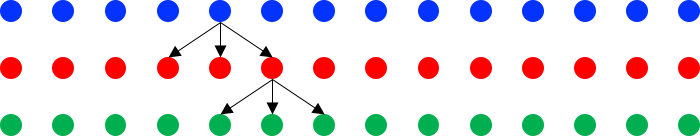
\includegraphics[height=0.45in]{TilingProcess/TilingProcess1.png}
		\caption{Original kernel iteration spaces and abbreviated dependences between iterations.}\label{tiling1}
	\end{subfigure}
	~
	\begin{subfigure}[t]{0.45\textwidth}
		\centering
		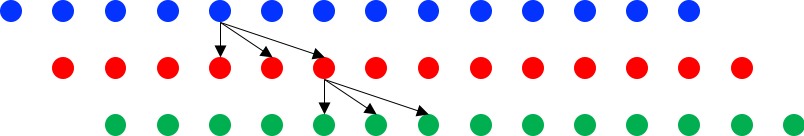
\includegraphics[height=.45in]{TilingProcess/TilingProcess2.png}
		\caption{After shifting kernels to remove negative dependences.}\label{tiling2}
	\end{subfigure}
	\par\bigskip
	\begin{subfigure}[t]{0.45\textwidth}
		\centering
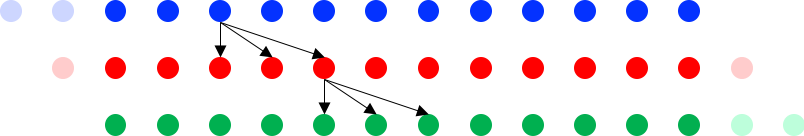
\includegraphics[height=0.45in]{TilingProcess/TilingProcess3.png}
		\caption{Shared iteration space. Chain could be fused sequentially.}\label{tiling3}
	\end{subfigure}
	~
	\begin{subfigure}[t]{0.45\textwidth}
		\centering
		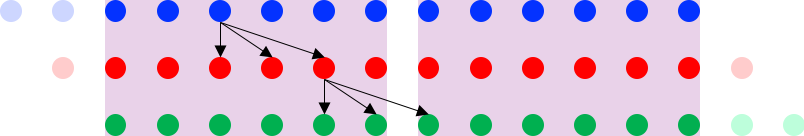
\includegraphics[height=.45in]{TilingProcess/TilingProcess4.png}
		\caption{Underlying tiles for TileSize=6 shaded in purple.}\label{tiling4}
	\end{subfigure}
	\par\bigskip
	\begin{subfigure}[t]{0.45\textwidth}
		\centering
		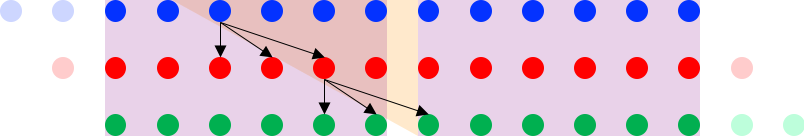
\includegraphics[height=0.45in]{TilingProcess/TilingProcess5.png}
		\caption{Overlap for each tile shaded in orange. Tiles against low edge have no overlap.}
	\end{subfigure}
	~
	\begin{subfigure}[t]{0.45\textwidth}
		\centering
		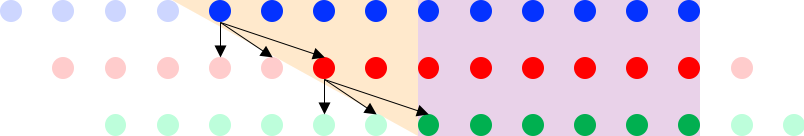
\includegraphics[height=.45in]{TilingProcess/TilingProcess6.png}
		\caption{An individual overlapped tile.}
	\end{subfigure}
	\par\bigskip
	\begin{subfigure}[t]{0.45\textwidth}
		\centering
		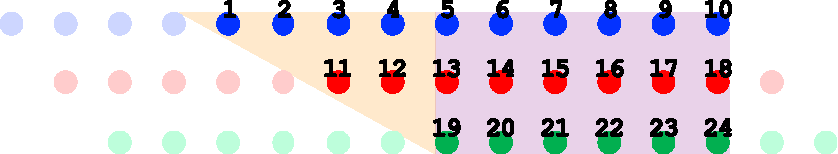
\includegraphics[height=0.45in]{TilingProcess/TilingProcess7.pdf}
		\caption{Execution order for an individual tile without fusion.}\label{tileNofuse}
	\end{subfigure}
	~
	\begin{subfigure}[t]{0.45\textwidth}
		\centering
		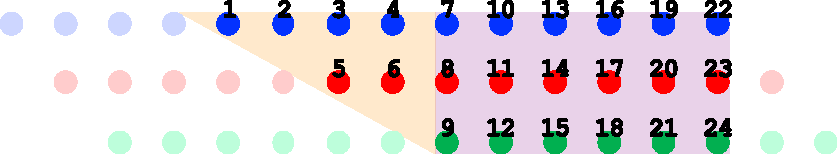
\includegraphics[height=0.45in]{TilingProcess/TilingProcess8.pdf}
		\caption{Execution order for an individual tile with fusion.}\label{tileFuse}
	\end{subfigure}
	\par\bigskip
	\begin{subfigure}[t]{\textwidth}
		\centering
		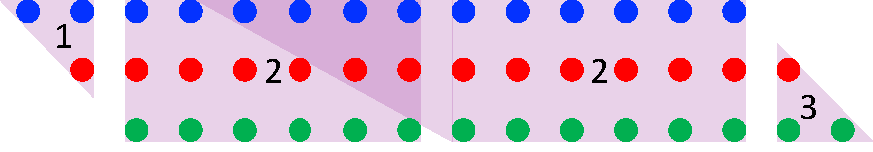
\includegraphics[height=0.45in]{TilingProcess/TilingProcess9.pdf}
		\caption{Global execution order for entire computation.}\label{tiling9}
	\end{subfigure}

\caption{Overlapped tiling of 3 one-dimensional loops.}\label{tilingProcess}
\end{figure*}

\section{Transformations Safety in RAJALC}
Section~\ref{sec:transspec} shows how a user can specify the use of loop fusion transformations
or overlapped and fusion transformations on loops in a chain.
In this section, I describe 
how RAJALC generates different execution schedules and uses the information gathered from the symbolic evaluation to verify their correctness.

\subsection{Loop Shifting for Stencil Computations}

While \verb.fuse_always. prescriptively apples a fusion transformation
without checking its legality, \verb.fuse. uses symbolic evaluation to
guide a legal loop fusion.
For a fusion to be legal, the inter-loop dependences cannot have a
negative direction.
However, loops can often be shifted to make such
dependences non-negative.
Figures~\ref{tiling1} and~\ref{tiling2} show an example of shifting the
loops to adjust negative dependences.
Prior work showed how to convert the dependence relations into constraints
of an ILP optimization problem~\cite{bertolacci2019using}.
RAJALC minimizes the sum of the non-negative shift amounts
$S_{1,1},S_{1,2},\ldots,S_{2,1},\ldots,S_{l,n}$ with the constraints $S_{b,i} + d_i \geq S_{a,i}$ for each dependence
$[d_1,d_2,\ldots,d_n]$ from kernel $a$ to $b$.
Solutions to this problem correspond to shift amounts that enable loop fusion.
RAJALC also use this shifting mechanism to simplify the dependences for overlapped
tiling.

While fusion in this circumstance improves data locality, it restricts
parallelism.
Because fusion combines iterations of different loops, dependences that
are originally between different loops become dependences between iterations
of the same loop. 
While wavefront parallelism may still be possible, overlapped tiling often
offers a better balance of parallelism and data locality~\cite{CathieSC14}.

\subsection{Iteration Space Alignment and Lambda Generation}
When performing optimizing transformations, kernel iteration spaces do not
always completely align. 
Misalignments can arise from differences in the original iteration spaces
or from shifts to remove negative dependences. 
While the iterations the loops in a chain have in common are executed by
the fused or tiled kernels, we also must generate extra kernels to execute
the unshared boundary iterations.

Figure~\ref{fusionPartition} illustrates the generation of these kernels
for one $d=3$ loop in a chain. 
First, RAJALC calculates the shared iteration space of the chain, using the
intersection of all kernel iteration spaces, which yields a $d$-dimensional
hyper-rectangle within each kernel's iteration space, as
Figure~\ref{sharedSpace} shows.
To account for the boundary iterations, RAJALC then partitions the loop's
iteration space, using the faces of the shared iteration space.
Figures~\ref{preshare} and~\ref{postshare} show the iteration spaces of the
$2*d=6$ boundary kernels for the 3D loop. 
This process generates $2*d*n$ boundary kernels across the $n$ loops in a
chain, plus the one fused/tiled kernel over the shared iteration space. 
RAJALC orders these $2*d*n+1$ kernels by loop and dimension to execute the low
boundary iterations, the shared iterations, then the high boundary iterations.

Each kernel requires an iteration space and a lambda describing the loop body. 
For the boundary iterations, RAJALC uses the original lambdas. 
For the shared iterations, a new lambda is generated based on the transformation. 
With fusion, the new lambda executes the sequence of original lambdas, performing one iteration of each loop.
With overlapped tiling, the new lambda executes each original lambda across its share of the tile, as shown in Figure~\ref{tileNofuse}.


\begin{figure}
	\captionsetup[subfigure]{justification=centering}
		\centering
		\begin{subfigure}[t]{0.33\textwidth}
			\centering
			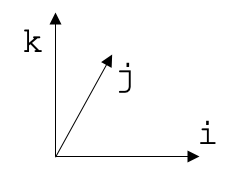
\includegraphics[height=0.5in]{FusionPartition/axes.png}
			\caption{Dimension order of loop.}
		\end{subfigure}
		
	%	\begin{subfigure}[t]{0.33\textwidth}
	%		\centering
	%		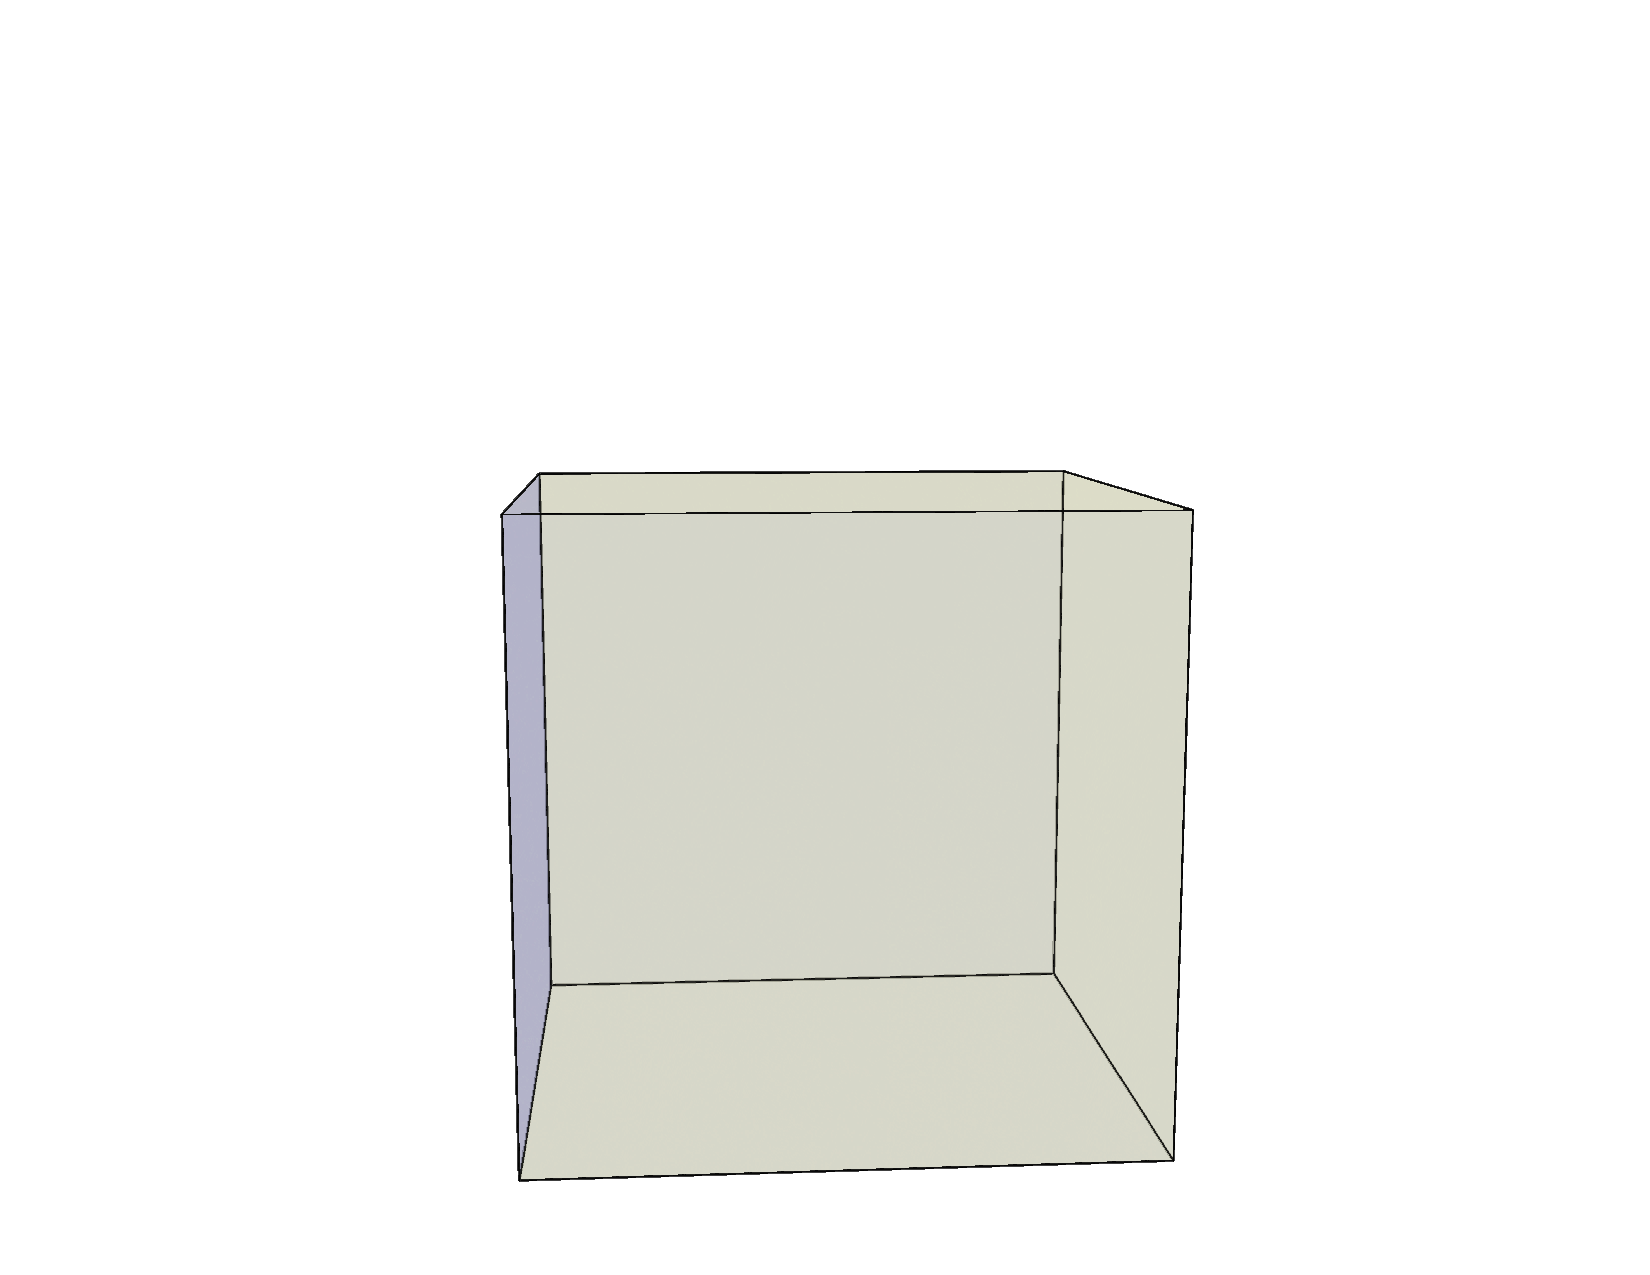
\includegraphics[height=1.5in, clip=true, trim=200 0 200 200]{FusionPartition/FusionPartition1.pdf}
	%		\caption{Original iteration space of one loop in chain.}
	%	\end{subfigure}
		
		\begin{subfigure}[t]{0.45\textwidth}
			\centering
			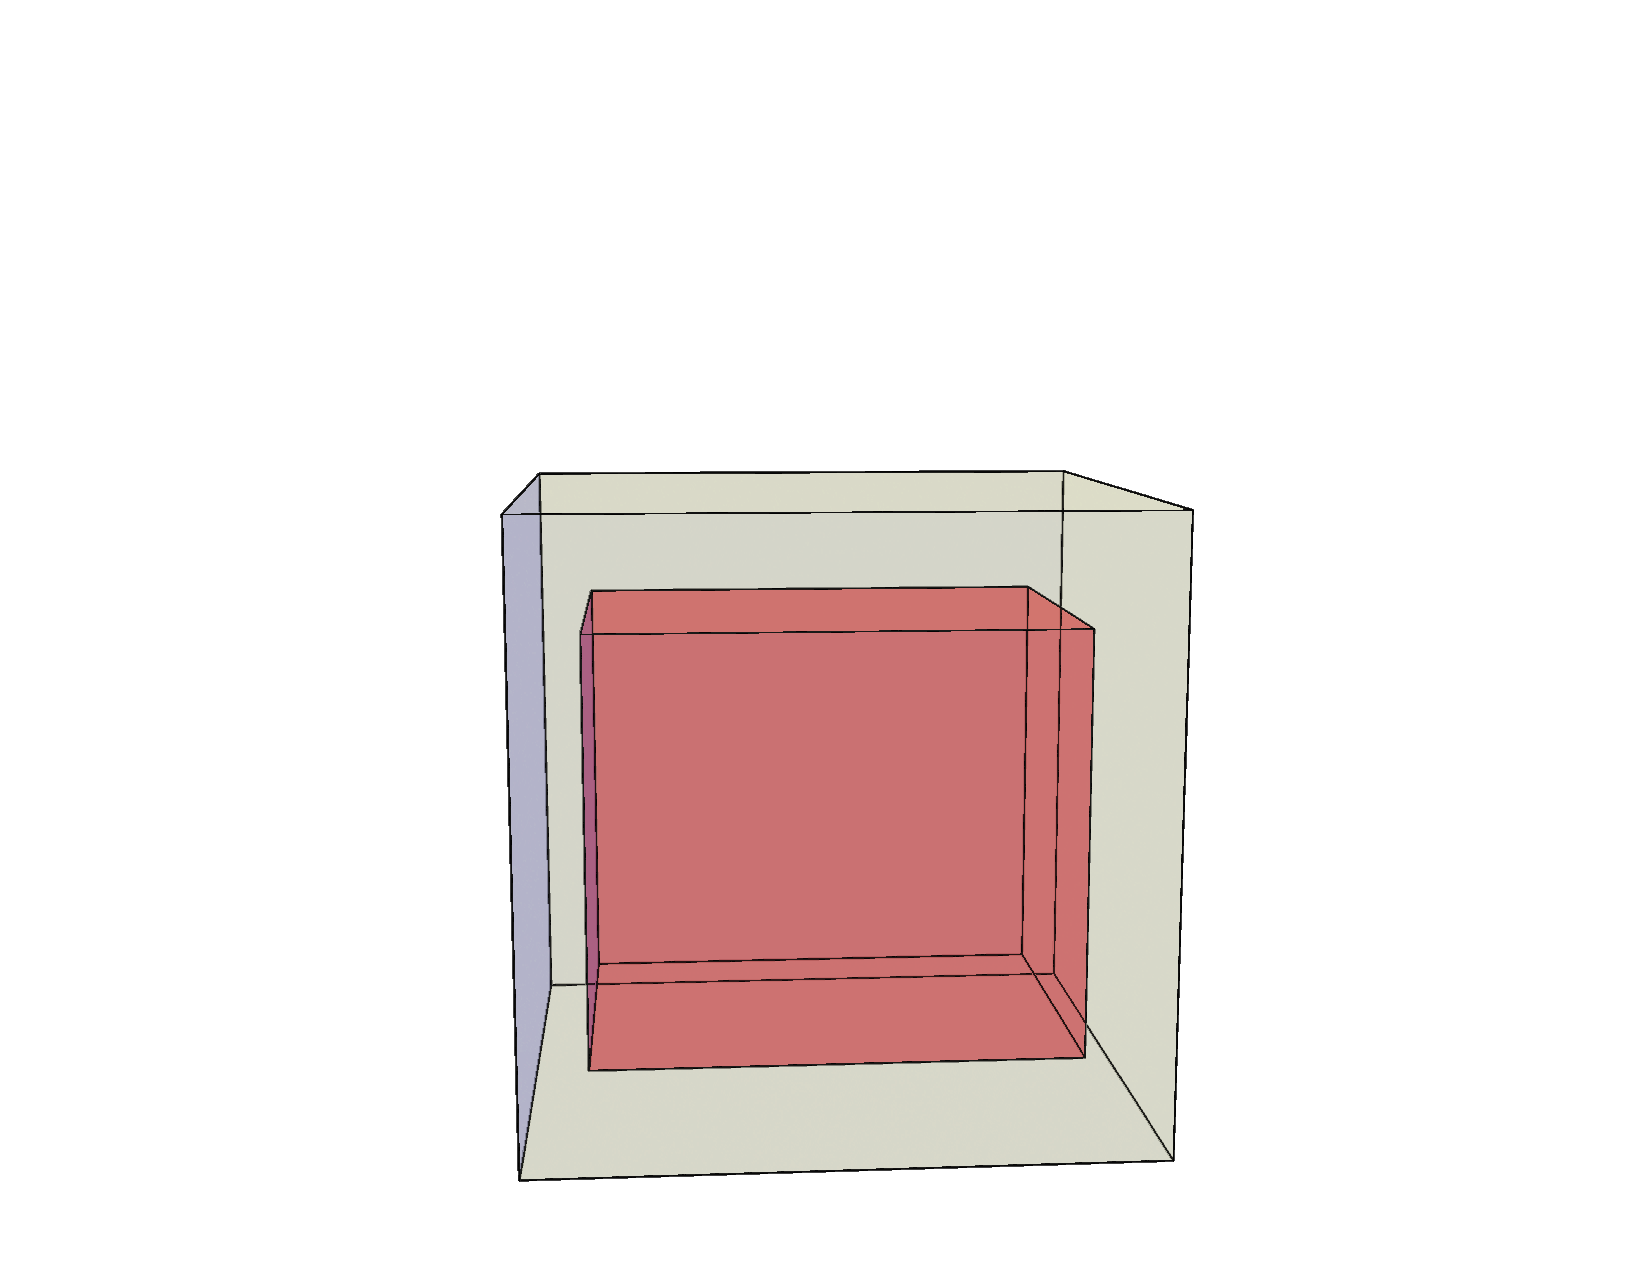
\includegraphics[height=1.5in, clip=true, trim=200 20 200 200]{FusionPartition/FusionPartition2.pdf}
			\caption{Original iteration space of one \\ loop in chain and shared iteration \\ space executed by fused kernel.}\label{sharedSpace}
		\end{subfigure}
		\begin{subfigure}[t]{0.45\textwidth}
			\centering
			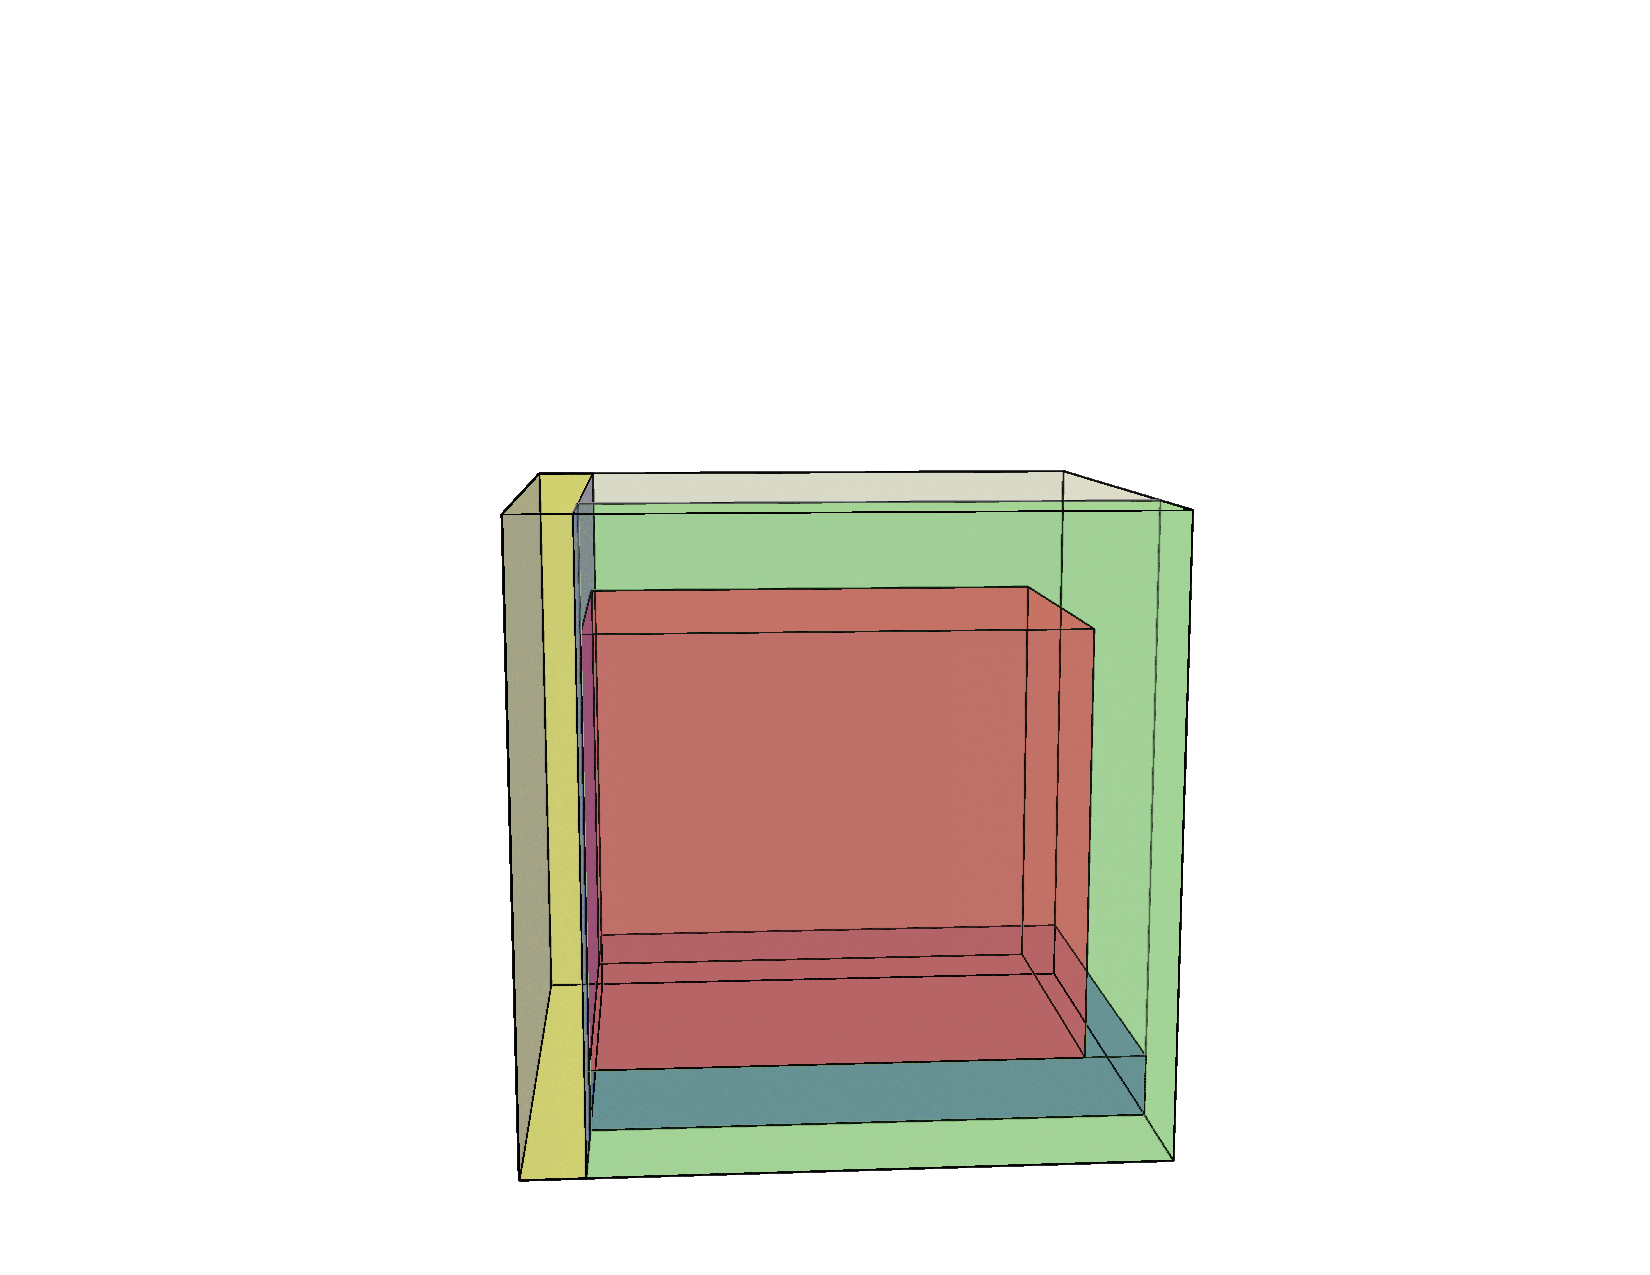
\includegraphics[height=1.5in, clip=true, trim=200 20 200 200]{FusionPartition/FusionPartition5.pdf}
			\caption{Lower boundary iteration spaces.}\label{preshare}
		\end{subfigure}
	
		\begin{subfigure}[t]{0.5\textwidth}
			\centering
			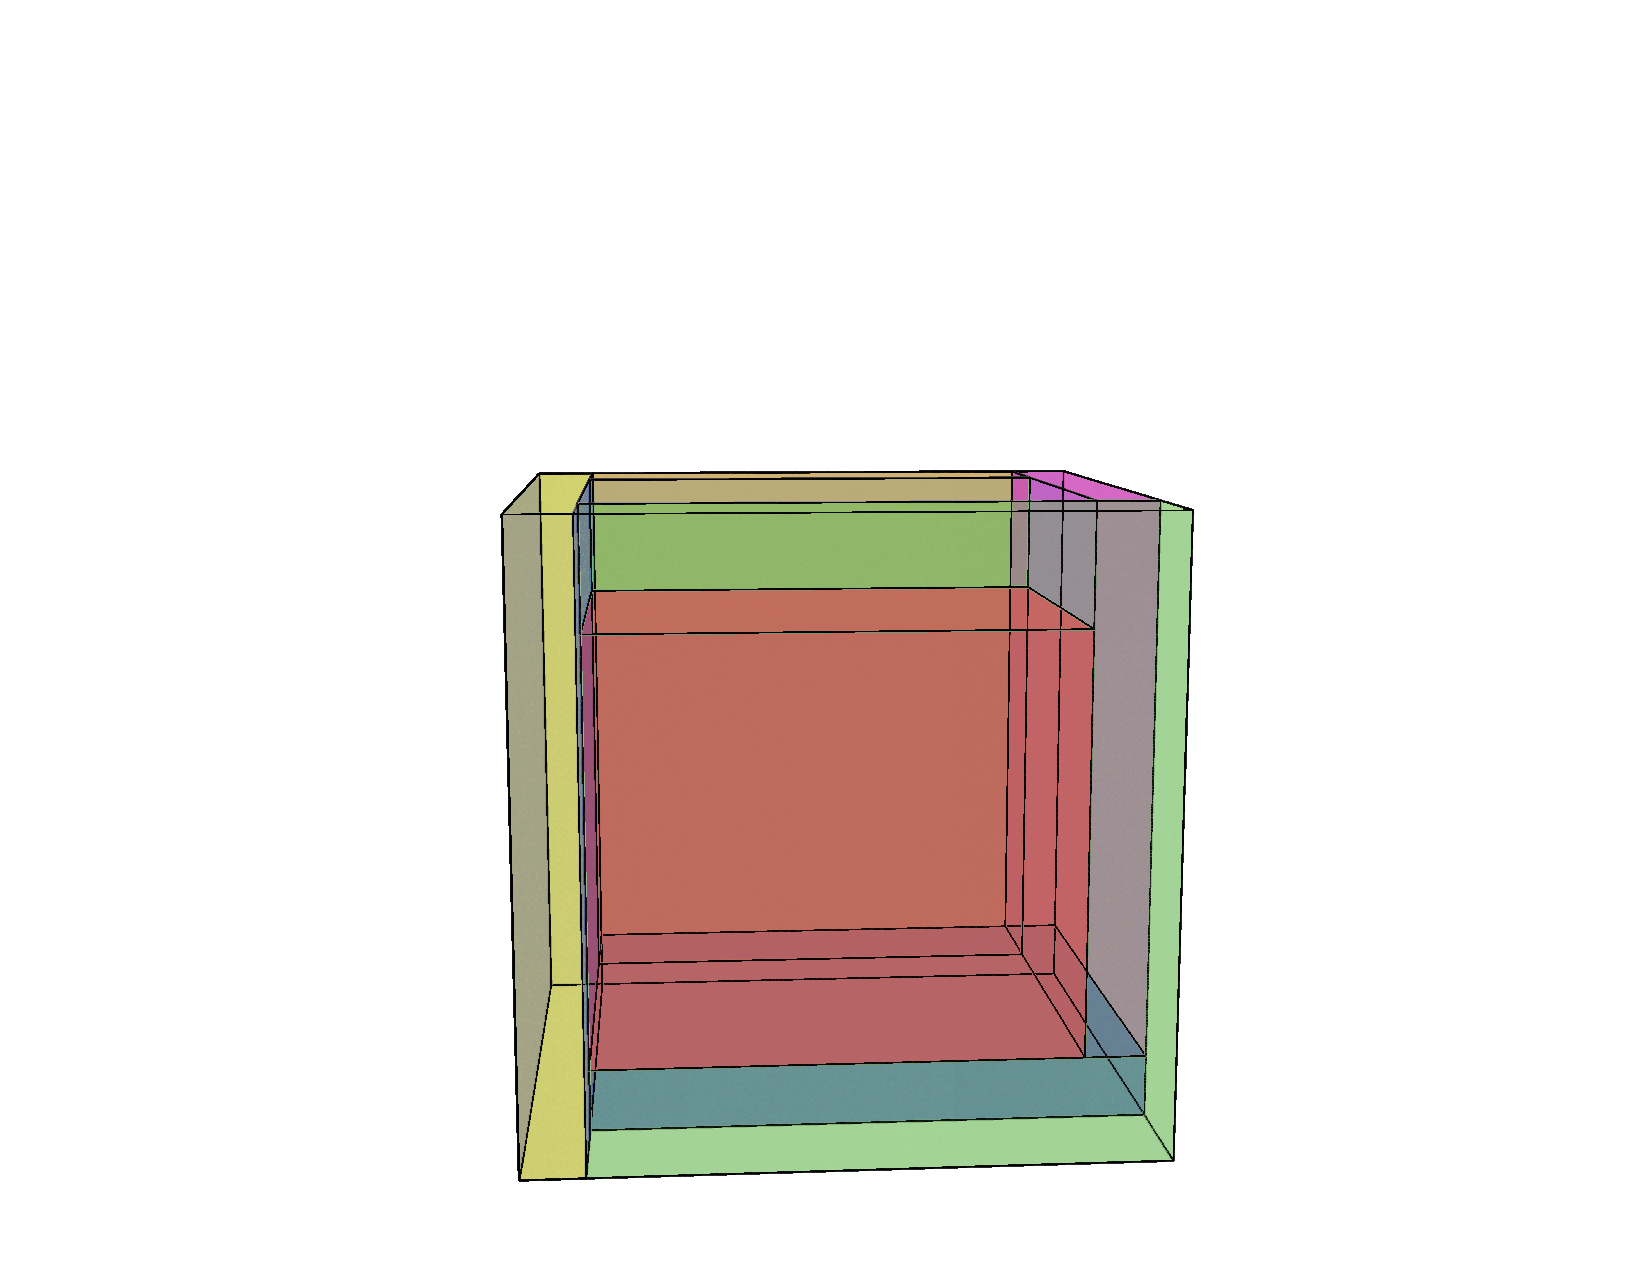
\includegraphics[height=1.5in, clip=true, trim=200 20 200 200]{FusionPartition/FusionPartition8.pdf}
			\caption{Higher boundary iteration spaces.}\label{postshare}
		\end{subfigure}
	\caption{Partitioning the iteration space of a single 3d loop. The original iteration space is $(0,10)\times(0,10)\times(0,10)$ and the fused iteration space is $(1,9)\times(2,8)\times(1,8)$. This partitioning process occurs for each kernel in the chain.}\label{fusionPartition}
	\end{figure}
	


\subsection{Overlapped Tiling}

Overlapped tiling proceeds similarly to the \verb.fuse. transformation. 
First, RAJALC calculates and applies shifts to remove negative dependences as
Figures~\ref{tiling1} and~\ref{tiling2} show.
Next, it calculates the overlapping iteration space and partition boundary
iterations as Figure~\ref{tiling3} shows.
Finally, it perform overlapped tiling as Figures~\ref{tiling4}-\ref{tiling9} show.

Before RAJALC can generate the kernel for the overlapped tiling, it must
calculate the overlap amounts. 
This is set up as an ILP optimization problem similarly to the calculation of the
shift amounts.
For $n$ kernels of dimension $m$, the optimization problem is over the $nm$
overlap amounts $O_{1,1},O_{1,2},\ldots,O_{2,1},\ldots,O_{n,m}$.
I introduce a non-negativity constraint to ensure that all overlap amounts
are greater than zero. 
I then add the constraints
$O_{a,1} >= O_{b,1} + d_{1}, O_{a,2} >= O_{b,2} + d_{2},\ldots,O_{a,m} >= O_{b,m} + d_{m}$
for each dependence $D=[d_{1},d_{2},\ldots,d_{m}]$ from kernel $a$ to kernel $b$,
which ensures that if a tile includes an iteration of kernel $b$, it also
includes all necessary iterations of kernel $a$.
Finally, it minimizes the sum of the overlap amounts
$\sum_{i=1}^{n} \sum_{j=1}^{m} O_{i,j}$.

After RAJALC calculates the overlap amounts, it generates a kernel that iterates
over each tile, executing the original kernels for the iterations of the tile.
The two overlapped tiling transformations, \verb.overlapped_tile_no_fuse.
and \verb.overlapped_tile_fuse. differ in their schedule for executing each
tile.
Without fusion, it executes the tile one kernel at a time: all of $knl1$ is
executed, then all of $knl2$, and so on. 
tile sizes are constrained for this schedule by cache size and by the size of
the overlap. 
Tiles must be small enough to fit into cache to maximize data locality
benefits, but tile size should be maximized to reduce the proportion of
recomputation.

In contrast, the \verb.overlapped_tile_fuse. transformation fuses iterations
within each tile using the fusion algorithm described above.
Introducing fusion into the tile decouples data locality from cache size.
Unrestricted by cache considerations, the only limit on tile size is the
need for parallelism, enabling larger tiles than otherwise possible.

\section{Case Study: RAJA Performance Suite}

I evaluate the advances through two case studies, porting the RAJA
Performance Suite (RAJAPerf)~\cite{hornung2017raja} and LULESH from
standard RAJA to RAJALC\@
In both case studies, I evaluate the performance and porting process
of the RAJALC implementations and I detail benefits and limitations
of the approach.

The RAJA Performance Suite is a collection of benchmark kernels that are
used to evaluate RAJA performance.
The suite contains 46 benchmark kernels across five categories; 33 contain
a single loop nest, leaving 13 kernels for which the advances are relevant.
Four of these are matrix computations involving reductions to which 
RAJALC's current capabilities do not apply. 
Finally, one benchmark does not exhibit any data reuse, so no data locality 
optimizations are relevant, including those supported here. 
Thus, I evaluate RAJALC on 8 benchmark kernels.

For each of the 8 kernels, I identify a locality-improving transformation
and implement new variants.
The first variant, \verb.Hand_Opt., applies the transformations directly.
The second variant, \verb.LoopChain., applies the transformation using RAJALC\@.
I record the number of modified or added source lines of code for each
variant and evaluate their performance on three systems.
%Rose
System Intel1 has an 8-core Intel Core i7--6900K CPU at 3.2 GHz and 32G of memory.
% 512K L1 cache, 2M L2 cache, and 20M L3 cache.
It runs Ubuntu 16.04.7 and GCC11.0.
%Quartz
System Intel2 has a 36-core Intel Xeon E5--2695 CPU at 2.1 GHz and 128 GB of memory.
%Lassen
System Power9 has an 44-core IBM Power9 at 3.5 GHz and 256 GB of memory.
Systems Intel2 and Power9 run TOSS 3 and GCC8.3.1.


\subsection{Benchmark Descriptions}

I categorize each benchmark as either point-wise or stencil. 
Point-wise loops access at most one element of each array per iteration,
while stencil loops access a fixed pattern of elements of each array per
iteration. 
The loop bodies
\verb.lambda1. and \verb.lambda2. in Listing~\ref{transformExample} are
examples of point-wise loops, while \verb.lambda3. and \verb.lambda4. are
examples of stencil loops.

Three of the benchmarks, \verb.GEN_LIN_RECUR., \verb.ENERGY., and
\verb.PRESSURE., are point-wise computations.
\verb.GEN_LIN_RECUR. comes from a general linear recurrence computation and
\verb.ENERGY. and \verb.PRESSURE. are loops extracted from LULESH, a
hydrodynamics code. 
For these benchmarks, loop fusion does not interfere with parallelism, so
I apply that transformation.

The other five benchmarks are stencil computations: \verb.JACOBI_1D.,
\verb.JACOBI_2D., \verb.HEAT_3D., \verb.HYDRO_2D., and \verb.FDTD_2D..
\verb.JACOBI_1D., \verb.JACOBI_2D., and \verb.HEAT_3D. compute solutions
to discretized PDEs in their respective dimensions.
\verb.HYDRO_2D. is part of a hydrodynamics code.
\verb.FDTD_2D. is a finite-difference time-domain kernel that is unique
among the stencil computations because I can fuse two of its four loops 
without inhibiting parallelism.
Thus, I apply that transformation.
The other four require shifting to be fused, so I apply overlapped tiling
to retain sufficient parallelism.

\subsection{Porting}

Implementing the fusion transformation is fairly easy. 
For the RAJALC variant, because I can confirm their point-wise nature
visually, symbolic evaluation is unnecessary.
Thus, I directly apply the transformation without converting the kernels to 
RAJA Views.
The hand-applied variant code changes are also low impact; in a real
application they would not be desirable as the kernels may be used separately
in other contexts.
Instead of multiple calls to \verb.RAJA::kernel. with the different loop
bodies, a single call is made with all loop bodies as one.
For the \verb.GEN_LIN_RECUR. benchmark, I also apply a loop reversal
transformation by hand to both variants. RAJALC does not currently support 
loop reversal, but its inclusion in the implementation would not be difficult.
However, automation of its use and its limited applicability in 
existing RAJA applications has made its implementation low priority. 

For \verb.HYDRO_2D., applying overlapped tiling transformation with RAJALC 
requires minimal changes: I add two lines of code and change three. 
In contrast, the hand implementation changes four lines and added 41
new lines, effectively an order of magnitude more effort. 
These additional lines calculate the amounts to shift and to overlap, 
create the new, tiled kernel, and execute the boundary iterations not
within the tiled area. 
These changes are not simple; the porting process encountered errors
in nearly all parts: shifting, boundary iterations, tile sizes, tile
bounds, and tile execution.

Porting effort in source lines of code
for the other three overlapped tiling kernels is similar to 
\verb.HYDRO_2D., with one major difference.  
While \verb.HYDRO_2D. has distinct input and output arrays; \verb.JACOBI_1D., 
\verb.JACOBI_2D., and \verb.HEAT_3D. each use one of two arrays for
input and output, which introduces anti-dependences that inhibit 
overlapped tiling. 
To mitigate this effect, I modify the kernels to use
a double-buffer strategy that eliminates the anti-dependence. 
Listing~\ref{jacobiDoubleBuffer} shows the double-buffer reference
implementation for \verb.JACOBI_1D..
%%
I add the double-buffer transformation by hand in these three variants;
its automation is future work.
I plan to use the access information collected during symbolic evaluation
to identify chains that require it and to implement the double buffer within
the View class.
\begin{figure}[t]
\begin{lstlisting}[label={jacobiDoubleBuffer},caption={Double-Buffer Implementation for JACOBI\_1D}]
for(int t = 0; t < numIters; t++) {
	temp = A1.data_ptr;
	A1.data_ptr = A2.data_ptr;
	A2.data_ptr = temp;
	for(int i = 0; i < length; i++) {
		B(i) = 0.33333 * (A1(i-1) + A1(i) + A1(i+1));
	}
	for(int i = 0; i < length; i++) {
		A2(i) = 0.33333 * (B(i-1) + B(i) + B(i+1));
	}
}
\end{lstlisting}
\end{figure}

Table~\ref{sloc} shows the number of changed and added source lines of code
for all benchmarks.
Overall, manual porting difficulty in source lines of code 
increases as the dimensionality of a 
kernel increases, mostly due to the specification of the boundary iterations. 
Alternatively, RAJALC porting difficulty is similar regardless of the loop
dimensionality.
Also, while with RAJALC code retains its original structure, the 
hand-implemented transformations obscure the underlying computation,
which significantly complicates code maintenance.
\begin{table}[t]
\begin{tabular}{|l|l|l|l|l|}
\hline
\textbf{Benchmark}       & \multicolumn{2}{l|}{\textbf{\begin{tabular}[c]{@{}l@{}}Manual \\ Implementation\end{tabular}}} & \multicolumn{2}{l|}{\textbf{\begin{tabular}[c]{@{}l@{}}RAJALC\\ Implementation\end{tabular}}} \\ \hline
\cellcolor[HTML]{9B9B9B} & Changed                                         & Added                                        & Changed                                        & Added                                        \\ \hline
\textit{ENERGY}          & 6                                               & 6                                            & 6                                              & 2                                            \\
\textit{PRESSURE}        & 2                                               & 3                                            & 2                                              & 2                                            \\
\textit{GEN\_LIN\_RECUR} & 1                                               & 1                                            & 2                                              & 2                                            \\
\textit{FDTD\_2D}        & 8                                               & 4                                            & 9                                              & 4                                            \\
\textit{HYDRO\_2D}       & 4                                               & 41                                           & 3                                              & 2                                            \\
\textit{JACOBI\_1D}      & 3                                               & 17                                           & 3                                              & 3                                            \\
\textit{JACOBI\_2D}      & 10                                              & 33                                           & 10                                             & 3                                            
\\
\textit{HEAT\_3D}        & 12                                              & 38                                           & 12                                             & 3                                            \\ \hline
\textit{Average}        & 5.8                                              & 17.9                                           & 5.9                                            & 2.6                                            \\ \hline
%\textit{Average}        & 5.75                                              & 17.875                                           & 5.875                                            & 2.625                                            \\ \hline
\end{tabular}
\caption{Lines of Code Impact (Excludes double-buffer transformation changes)}\label{sloc}
\end{table}

\subsection{Performance}
\begin{figure}
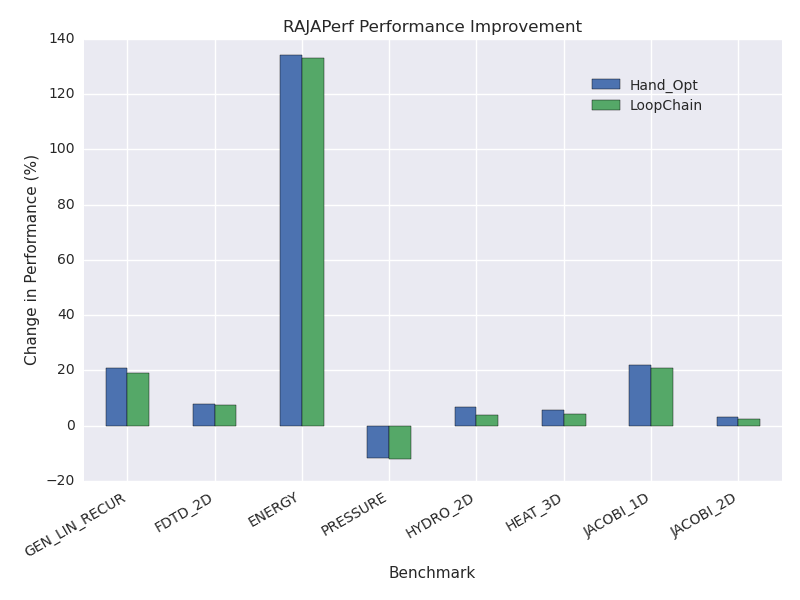
\includegraphics[width=\linewidth]{results/RajaPerf/Rose/RAJAPerf.png}
\caption{Performance changes of RAJAPerf benchmarks on System Intel1 (higher is better).}\label{RAJAPerfPerf}
\end{figure}
Figure~\ref{RAJAPerfPerf} shows the performance of the hand-implemented
and RAJALC variants relative to the original implementations on System Intel1. 
For the double-buffer implementations, I show the performance relative to an 
un-transformed double-buffer implementation. 
I report the average of ten runs. 

For the fused benchmarks, \verb.GEN_LIN_RECUR. and \verb.FDTD_2D. improve
modestly while \verb.PRESSURE. performance drops slightly, likely due to low amounts of data reuse. 
\verb.ENERGY. runs more than two times faster than the original, likely due
to the larger number of fused kernels than the other benchmarks. 
For all four, the RAJALC variant's performance is comparable to the
hand-implemented loop fusion. 
 
For the overlapped tiled benchmarks, the \verb.Hand_Opt. variant improves
performance up to 22\% for all benchmarks.
The RAJALC variant, which achieves its best performance with different tile sizes, improves performance by 
up to 20\%.
For both variants, the tile sizes were tuned manually.
Overall, the RAJALC variant achieves 85\% of the geometric mean performance
improvement of the hand-implemented variant. 


Because of the large thread counts on Systems Intel2 and Power9, I evaluated the scaling performance of RAJAPerf when using RAJALC\@.
Unlike on System Intel1, RAJAPerf often did not benefit from the inter-loop
optimizations on Systems Intel2 and Power9, even when applied by hand. 
However, the direction of RAJALC's performance impact was nearly identical to the hand-optimized code. 
On System Intel2, 47 of the 48 benchmark-thread-count combinations had the same direction of impact.
On System Power9, all 48 combinations matched the direction of performance impact between the two variants.
Overall, the geometric mean of the fraction of the hand-implemented speedup achieved by RAJALC ranges across thread counts from 0.92 and 0.97 on System Intel2 and 0.95 and 1.02 on System Power9. 
This is evidence that RAJALC is a useful tool for quickly prototyping transformations without large refactoring costs and accurately recreates the performance impact of hand implementing the transformations.

\section{Case Study: LULESH}

While the RAJAPerf case study demonstrates the types of computations RAJALC
can optimize, the second case study, LULESH, explores its potential within a
larger application.
LULESH is a DOE proxy application for shock hydrodynamics codes.
It solves a simple Sedov blast problem using the typical numerical algorithms and computational characteristics for larger codes.

As with the previous case study, I characterize the porting process and
evaluate RAJALC performance compared to the original implementation.
For this evaluation, I ported LULESH v2.0~\cite{LULESH2}. 

\subsection{Porting}

Porting LULESH is more involved than the RAJAPerf kernels. 
I must first identify the part of the application to optimize,.
I choose the function \verb.EvalEOSForElems., which has a long series
of point-wise computations over the same iteration space.
The \verb.ENERGY. and \verb.PRESSURE. benchmarks within RAJAPerf are
from this part of LULESH\@.

\subsubsection{Code Change: Arrays to Views}

The RAJA implementation of LULESH uses RAJA execution statements, but
does not use RAJA Views for arrays and vectors. 
Thus, I first convert these data structures to use Views.
For many of the data structures, array accesses are abstracted through
indexing functions. 
I replace these indexing functions directly with Views without changing
the source code of the algorithms.
However, the existing version often uses arrays, especially for local and
temporary storage.
I wrap these arrays with Views and change the accesses from brackets to
parentheses, a tedious but simple code change.

\subsubsection{Code Change: Kernel Objects}

The second required change uses RAJALC kernel objects instead of direct
code execution.
I move the series of point-wise computations in \verb.EvalEOSForElems. that operate over the same iteration space into many individual functions.
I modify them to create and to return the kernel objects, which allows us
to fuse them, both by hand and with RAJALC\@.


\subsubsection{Challenge: Indirect Accesses}
The \verb.nodelist. function, which creates a list of indices for the area
around an element, poses a challenge to the LULESH porting.
Because this function takes the loop index and returns a list of indices,
it interferes with symbolic evaluation.
RAJALC has similarities to inspector-executor strategies commonly used when optimizing sparse codes, which may provide some direction in attempts to optimize RAJA-based sparse codes. 

\subsubsection{Challenge: Non-contiguous Iteration Spaces}

LULESH is an unstructured application: its iteration spaces are collections
of ranges instead of contiguous ranges. 
For example, instead of iterating over every value from 0 to 100, it may
iterate over values 0 to 10, then 17 to 23, then 52, 73, and 75 to 100.
RAJALC currently only handles contiguous iteration spaces, so it only
applies fusion to LULESH problems that use contiguous ranges.
In practice, this limitation is a benefit over hand optimizations that assume
such ranges.
Nonetheless, the prevalence of unstructured scientific applications makes
fusion of unstructured ranges a valuable future research direction.


\subsection{Performance}

WIe evaluate the performance of three LULESH variants: Original, RAJALC, and
By Hand.
Original is the original v2 RAJA implementation.
RAJALC is the version ported to apply loop fusion with RAJALC while By Hand
directly applies loop fusion by hand.


\begin{figure}[t]
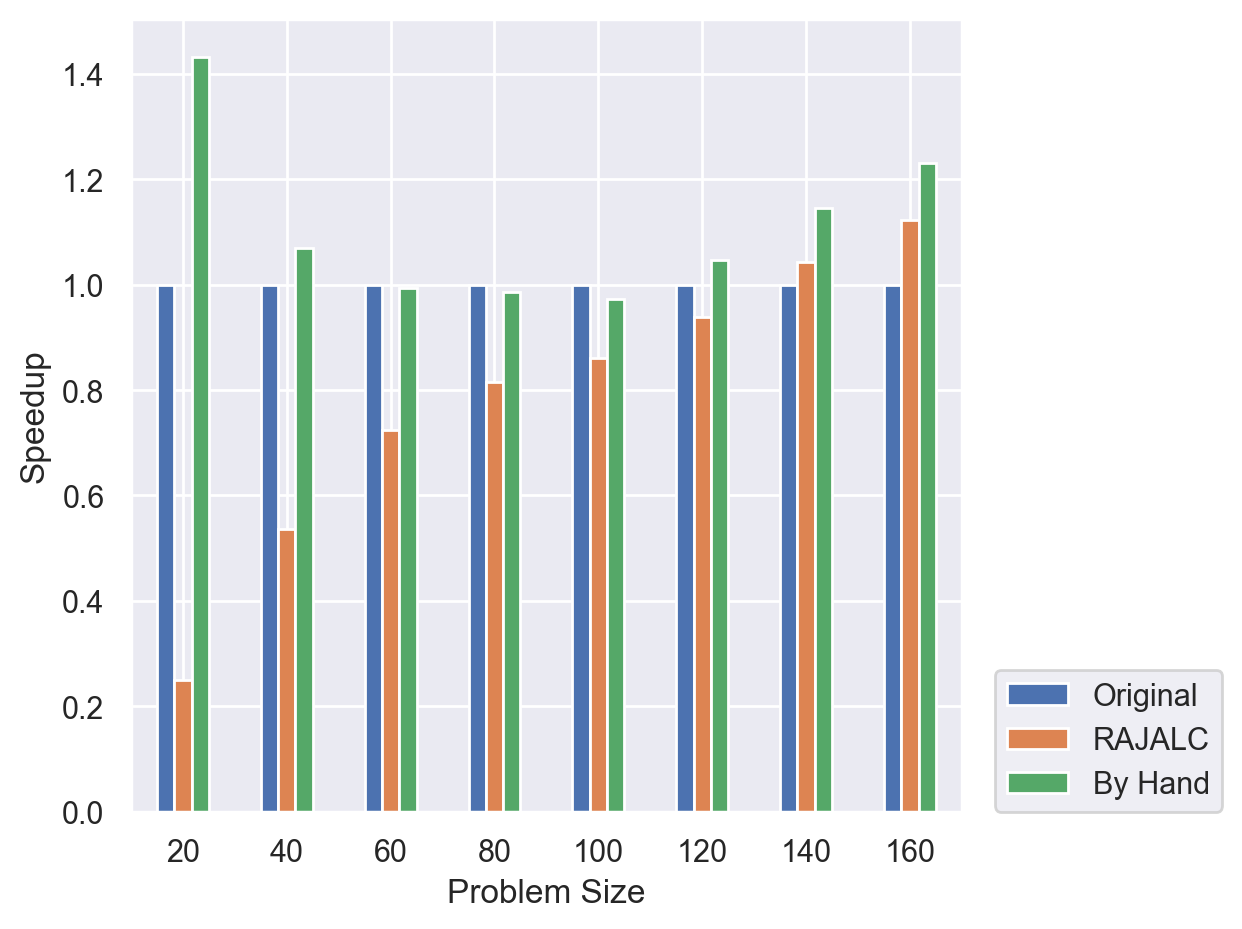
\includegraphics[width=\linewidth]{results/Lulesh/LuleshRoseGcc8All/LuleshRoseGcc8All.png}
\caption{LULESH Speedup on System Intel1 (higher is better).}\label{LULESHRose}
\end{figure}

\begin{figure}[t]
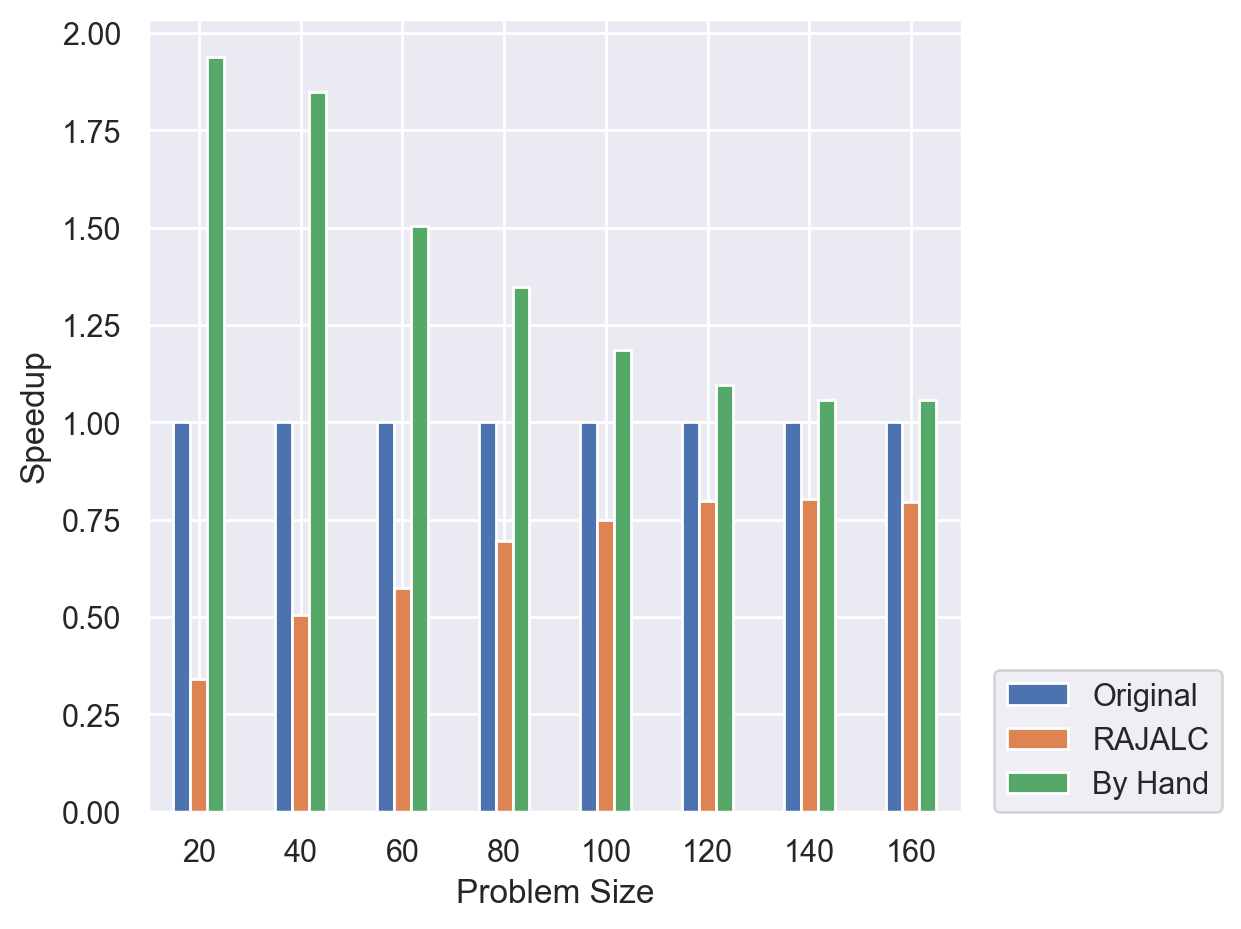
\includegraphics[width=\linewidth]{results/Lulesh/LuleshQuartzGcc8All/LuleshQuartzGcc8All.png}
\caption{LULESH Speedup on System Intel2 (higher is better).}\label{LULESHQuartz}
\end{figure}

\begin{figure}[t]
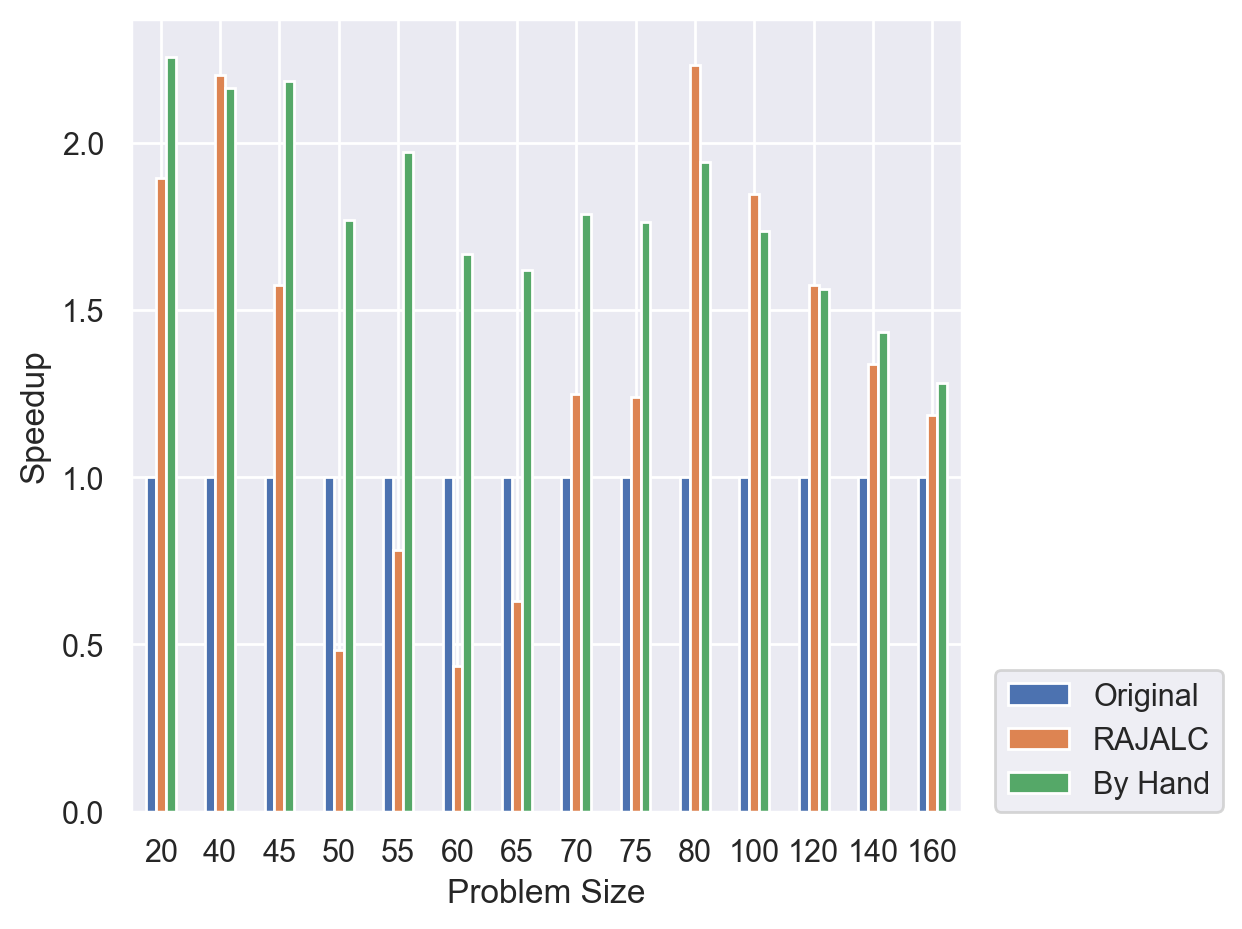
\includegraphics[width=\linewidth]{results/Lulesh/LuleshLassen/LuleshLassen.png}
\caption{LULESH Speedup on System Power9 (higher is better).}\label{LULESHLassen}
\end{figure}

Figures~\ref{LULESHRose},~\ref{LULESHQuartz}, and~\ref{LULESHLassen} show
the average speedup over three runs relative to Original for several problem
sizes. 
For the recommended problem sizes on Systems Intel1 and Intel2, RAJALC does
not see performance improvements, but By Hand does.
I expect improvement since the fused kernels are the same as \verb.ENERGY.
and \verb.PRESSURE. in RAJAPerf.
I examine the generated code with OptVis~\cite{devkota2020ccnav}, to uncover
two likely culprits.
First, although the RAJALC code includes inlining directives, some calls
within the fused kernel were not inlined. 
In the By Hand variant, the calls are always inlined by virtue of the code
being combined into a single lambda. 
Introducing multiple extra calls each iteration of the fused loop likely
contributes to the performance degradation with RAJALC\@
Second, the code for the kernels that were successfully inlined is dispersed
throughout the binary and contains more than twice as many basic blocks as
the By Hand variant. 
These extra jumps, often to completely different parts of the binary, also
likely reduce RAJALC performance. 
One method to reduce the first effect has been addressed by the authors 
in an OpenMP feature proposal. Modern compiler inlining directives are generally 
only suggestions to the compiler. A standardized, forced inlining directive would 
reduce the problem of extra calls within the kernel.
However, the implementation makes use of forced inlining directives, 
so future work will examine why these directives are not leading to the expected binary structure.

System Power9 exhibits much larger performance improvements, including at small
problem sizes. 
However, there is anomalous results for RAJALC for problem sizes around 60. 
I include additional problem sizes for System Power9 to contextualize this drop in performance. 
While not as significant, there is also volatility in the hand-implementation performance for these problem sizes.

\section{Related Work}

Several other approaches provide performance-portable loop optimization.
Inter-loop optimization has been studied for decades, but usually
within the context of domain-specific languages (DSLs).
This work aims to enable more general approaches within the performance portability library framework.

\subsection{Portable Intra-Loop Optimization}
RAJA~\cite{hornung2014RAJA}, OpenMP~\cite{OpenMPver5}, Kokkos~\cite{edwards2014kokkos},
and SYCL~\cite{SYCL2019} provide ways to parallelize and provide data locality
within individual loops.
For performance portability, Pennycook et al.~\cite{Pennycook2018} show an
example  that uses OpenMP to have a single source code with specializations
in pragmas to target different architectures.

%[Cuda has a way to schedule kernels in a queue so that data can be shared between
%those kernels?]  FIXME

Active libraries~\cite{VeldhuizenActive98} such as the 
Matrix Template Library~\cite{Siek:1999:SPM},
Blitz++~\cite{Veldhuizen2000},
and the Bernoulli compiler~\cite{ahmed2000framework,kotlyar1997relational} fuse some
computations using expression templates, but cannot fuse across statements.

\subsection{By Hand Inter-Loop Optimization}
Some work has experimented with overlapped tiling and other inter-loop
scheduling by hand.
Olschanowsky et al.~\cite{CathieSC14} showed that scheduling across loops and
reducing the temporary storage requirements led to problem size scaling and
significantly better performance in a CFD application.
Wahib and Maruyama~\cite{Wahib14} showed the importance of fusing kernel
computations for GPU execution.

Numerous approaches to scheduling across an outer ``time loop'' in a stencil
code have been investigated as early as 1998~\cite{Bassetti98,Wonnacott00}.  
The Cactus project~\cite{Ripeanu2001,Allen00cactus-gtoolkit} and 
Ding and He~\cite{Ding2001} demonstrated  overlapped tiling by expanding
ghost cells in stencil computations. 
Wonnacott and Strout~\cite{Wonnacott13} review many other approaches to
time tiling for PDE codes that do explicit stepping versus implicit stepping.

\subsection{DSLs Providing Inter-Loop Optimization}
A number of DSLs have been developed for specifying and
optimizing stencil computations.
The Pochoir work~\cite{Tang2011} embedded cache oblivious performance
optimizations to improve temporal locality in C++ code.
STELLA~\cite{Gysi2015}  and YASK~\cite{YASK2016} can specify and 
tune 3D finite difference stencil computations.
Rawat et al.~\cite{Rawat18} present a DSL called StencilGen for specifying
stencil computations.
They present algorithms that perform overlapped tiling within stencil
computations and heuristics for fusing between the computations for GPUs.
Their work demonstrates some possible performance benefits of scheduling
across stencil computations when targeting GPUs and CPUs. In contrast,
I present ways to enable and to control these optimizations across loops
in the context of a more general, parallel library, specifically RAJA\@.

LIFT~\cite{Hagedorn2018} is a data parallel, functional intermediate
representation that supports dense computations and stencil computations.
Once a computation written in a DSL is transformed to LIFT, pattern-based
transformation can implement optimizations such as overlapped tiling and
target many different architectures.
Krishnamoorthy et al.~\cite{krishnamoorthy2007effective} present an automated tiling
technique for stencil computations in which neighboring tiles perform
overlapping computations, which reduces communication and improves load
balance.

%[Image processing pipelines, which are also stencil applications.  
Embedded DSLs for image processing pipelines, such as
Halide~\cite{ragan-kelley2013halide} and
PolyMage~\cite{mullapudi2015polymage}, support orthogonally specifying and
scheduling stencil computations.
By exposing separate mechanisms for scheduling them, PolyMage supports
various scheduling, fusion, and tile size selection
algorithms~\cite{Mullapudi2016,Jangda2018,Adams2019}.
%BRANDON: Adding differentiation
However, using these embedded DSLs limits the expressible computation and requires prohibitive porting costs for large applications.
%Jangda and Bondhugula~\cite{Jangda2018} have developed heuristics for selecting tile sizes and
%fusing across image processing pipelines.
%[Compiler techniques that schedule across loops.  Requires code to be quite simple to be analyzed and 
%there have been a number of different heuristics for deciding when to fuse.]

%[DNNs optimizing across loops]
Several DSLs that specify deep learning neural network
architectures, including Halide extended for reverse mode automatic
differentiation~\cite{Li2018}, Tensor Comprehensions~\cite{Vasilache2018},
TVM~\cite{TVM2018} and Latte~\cite{TruongLatte2016} optimize across loops.
These DSLs have specific approaches to scheduling such as the Halide scheduling
algorithm for DNN~\cite{Yang2020}.
AutoTVM in TVM~\cite{Chen2019} learns how to schedule.
Frameworks like Delite~\cite{Sujeeth2014} for developing DSLs support 
cross-computation scheduling.

Although the DSL approach can better target a particular application domain,
this work schedules across loops within RAJA supports a broader class of
applications.
Further, I provide a different separation of concerns. RAJA handles
performance portability while the loop chain extension handles scheduling
across loops.
DSL approaches handle all of the scheduling and targeting of architectures,
which leads to not all architectures being covered in some cases.

\subsection{Traditional Compiler Approaches}

Loop optimizations are used in a wide variety of compilers.
Polyhedral optimizations have been incorporated into production compilers with Graphite~\cite{trifunovic2010graphite} and Polly~\cite{grosser2011polly}.
Both works have similar approaches, starting by extracting polyhedral representation from an intermediate representation. 
Graphite works on the GNU GIMPLE representation and Polly on LLVM-IR\@.
After extracting polyhedral representations, they perform a number of analyses and transformations and regenerate new, optimized code.
Both approaches are general-purpose, automatic approaches.

PLuTo~\cite{bondhugula2008pluto} is another example of an automatic optimizing compiler. 
While Graphite and Polly perform optimizations as they lower from code to executable, PLuTo is a source-to-source optimizer. 
While it focuses on balancing parallelism and locality through loop tiling, PLuTo also has the ability to fuse producer-consumer loops. 
PLuTo searches a large space of possible tilings, but it does so automatically, leaving minimal room for the developer to select their own transformations.

Other approaches like AlphaZ~\cite{yuki2012alphaz} and CHiLL~\cite{tiwari2009scalable} provide scripting languages that iteratively transform loops in the program. 
The programmer writes an additional file containing the transformations they want applied to loops in the program such as permute, tile, or unroll. 
While these approaches allow more flexibility in transformation and maintain the original structure of their code, they introduce an additional stage in the toolchain.
A similar drawback applies to embedded DSLs that use their own compilers, such as Tiramisu~\cite{baghdadi2019tiramisu}.




%%%%%
\subsection{Staging and Other Loop Chain Approaches}

The most related work to this submission is work that gathers representations of computations and other work that aims to specify and optimize loop chains.
Lightweight modular staging~\cite{LMS2012} presented an approach for gathering 
a representation of computation to enable scheduling across that implementation
in Scala.

Bertolacci et al.~\cite{Bertolacci2016,bertolacci2019using} propose extensions to
OpenMP pragmas to express and schedule loop chains.
The approach requires annotations about data accesses in the pragmas.
That work enables the specification of loop fusion and wavefront tiling. 

Luporini et al.~\cite{Luporini2019} has a similar goal of enabling the source
code that uses a library  (in this case Devito~\cite{Luporini2018}) to
schedule across loop computations that share data.
The loops in their case have indirect array accesses.
Thus grouping computations to improve data locality requires a run-time
inspection phase~\cite{Strout14IPDPS}.
Luporini et al.\ use various Python library interfaces to specify computations
using per-loop modularization and then a lazy-computation step that gathers
the loop descriptions and generates inspector-executor code for performing 
sparse tiling.
%% BRONIS: The following does not seem necessary; is not discussed
%% \begin{verbatim}
%%    with loop_chain(name, tile_size, fusion_scheme, ...):
%%        <some PyOP2 parallel loops>
%% \end{verbatim}

The key differences between their work and this one is that I leverage the view 
capability of RAJA to avoid needing to annotate how data is being accessed
in each loop.  
Instead, symbolic analysis collects that information.

\section{Conclusion}
Inter-loop optimizations have long been known to improve data locality and 
to reduce synchronization costs of computations with loops the share data
with producer-consumer relationships.
However, the required refactoring has remained a tedious manual process with 
significant impact on code maintainability.
We have presented a design that retains the loop-based modularization typical
of scientific codes while enabling the automated application of important
inter-loop optimizations.
RAJALC adds a loop chain construct and some API parameters to enable symbolic
analysis of data access patterns in the RAJA performance-portability C++
library. 
Importantly, their use entails minimal code changes. 


